\chapter{Supplementary Results}
\label{app:supplementary}

This appendix reports the analyses that check the results of
Chapter~\ref{ch:evaluation} without changing them. All genre scores are film-level
macro-$F_1$ on the five-genre subset unless stated otherwise.

% =============================================================================
\section{All Paired Comparisons}
\label{sec:app_comparisons}

Table~\ref{tab:power_cmp_full} extends Table~\ref{tab:power_cmp} to every paired
comparison that was run on the five-genre subset.

\begin{table}[tbp]
  \centering
  \small
  \caption{All paired comparisons on the five-genre subset: film level, with the clip-level tests beside it.}
  \label{tab:power_cmp_full}
  \setlength{\tabcolsep}{3pt}
  \resizebox{\textwidth}{!}{%
  \begin{tabular}{lrcrr@{\hspace{10pt}}rrrr}
    \toprule
    & \multicolumn{4}{c}{Film level} & \multicolumn{4}{c}{Clip level} \\
    \cmidrule(lr){2-5} \cmidrule(lr){6-9}
    Comparison & $\Delta$ & 95\,\% CI & $p_{\text{boot}}$ & won & $\Delta$ & $p_{\text{boot}}$ & $p_{\text{NB}}$ & $p_{\lim}$ \\
    \midrule
    Emotion vs.\ VGGish           & $+0.093$ & $[-0.001,\,+0.191]$ & $0.052$ & 9 & $+0.039$ & $\mathbf{0.013}$ & $0.086$ & $0.069$ \\
    Emotion vs.\ AST              & $+0.139$ & $[+0.060,\,+0.222]$ & $\mathbf{<0.001}$ & 10 & $+0.037$ & $0.106$ & $0.223$ & $0.200$ \\
    Emotion vs.\ CLAP             & $+0.071$ & $[-0.022,\,+0.174]$ & $0.156$ & 9 & $+0.049$ & $\mathbf{0.019}$ & $0.102$ & $0.083$ \\
    Emotion vs.\ MusiCNN          & $+0.065$ & $[-0.039,\,+0.170]$ & $0.241$ & 9 & $+0.046$ & $\mathbf{0.040}$ & $0.112$ & $0.092$ \\
    Emotion vs.\ MIR              & $+0.094$ & $[+0.022,\,+0.174]$ & $\mathbf{0.010}$ & 10 & $+0.042$ & $\mathbf{0.044}$ & $0.196$ & $0.173$ \\
    Emotion vs.\ wav2vec 2.0      & $+0.196$ & $[+0.128,\,+0.265]$ & $\mathbf{<0.001}$ & 10 & $+0.076$ & $\mathbf{<0.001}$ & $\mathbf{0.031}$ & $0.021$ \\
    Emotion vs.\ PCA-8 control    & $+0.070$ & $[-0.011,\,+0.158]$ & $0.089$ & 10 & $+0.042$ & $\mathbf{0.020}$ & $0.151$ & $0.129$ \\
    \midrule
    Emotion vs.\ ground truth     & $-0.032$ & $[-0.090,\,+0.021]$ & $0.277$ & 0 & $-0.010$ & $0.340$ & $0.489$ & $0.468$ \\
    Ground truth vs.\ CLAP        & $+0.103$ & $[+0.011,\,+0.199]$ & $\mathbf{0.019}$ & 10 & $+0.059$ & $\mathbf{0.002}$ & $\mathbf{0.009}$ & $0.005$ \\
    PCA-8 vs.\ VGGish             & $+0.023$ & $[-0.042,\,+0.086]$ & $0.488$ & 7 & $-0.003$ & $0.885$ & $0.996$ & $0.996$ \\
    AST vs.\ CLAP                 & $-0.068$ & $[-0.129,\,+0.018]$ & $0.096$ & 2 & $+0.011$ & $0.561$ & $0.682$ & $0.668$ \\
    \bottomrule
  \end{tabular}}
\end{table}

In Table~\ref{tab:power_cmp_full}, $\Delta$ is the first route minus the second, and
``won'' counts the ten repeats in which the first route scores higher. The clip-level
block scores the same predictions over clips with the film bootstrap ($p_{\text{boot}}$)
and the Nadeau--Bengio corrected resampled $t$-test ($p_{\text{NB}}$); $p_{\lim}$ is the
smallest $p_{\text{NB}}$ this dataset allows with an unlimited number of repeats. Bold
marks $p<0.05$.

\subsection{Why the Nadeau--Bengio Test Stays Borderline}
\label{subsec:statistical_power}

The film bootstrap resamples the test films with the trained models held fixed and asks
how much a difference depends on which films make up the dataset. The Nadeau--Bengio test
\citep{nadeau2003inference} also charges for the variation that comes from which films were
used for training, and so it is the more conservative test. Only the $1/n$ term of its
corrected variance shrinks as repeats are added, so for a given dataset the attainable
$p$-value has a floor, $p_{\lim}$. For every borderline clip-level comparison of the
emotion route that floor lies above 0.05 (0.069 to 0.200). Additional repeats could
therefore never make these comparisons significant under this test; only more films could.

% =============================================================================
\section{Choice of Metric and Stability}
\label{sec:eval_robustness}

\subsection{Does the Choice of Metric Matter?}

Multi-label classification has no single natural metric \citep{sokolova2009systematic}.
Table~\ref{tab:metric_family} scores the emotion route, the two strongest direct
representations of the clip-level analysis and the PCA-8 control under a wider family of
metrics, and Figure~\ref{fig:metric_family} shows the most informative of them as the
distance of each route above the base-rate random guess of that metric. Apart from the
first row, all metrics are computed over clips, from the same predictions.

\begin{table}[tbp]
  \centering
  \small
  \caption{The routes under thirteen metrics on the five-genre subset (seed 42, mean of ten repeats).}
  \label{tab:metric_family}
  \setlength{\tabcolsep}{3.5pt}
  \resizebox{\textwidth}{!}{%
  \begin{tabular}{lrrrrrrr}
    \toprule
    Metric & Emotion & VGGish & AST & PCA-8 & Most freq. & Random & $\Delta$ ($p$) \\
    \midrule
    \multicolumn{8}{l}{\emph{Genres weighted equally, decision at 0.5}} \\
    Macro-$F_1$ over films            & \textbf{0.460} & 0.367 & 0.318 & 0.390 & 0.168 & 0.309 & $+0.093$ (0.063) \\
    Macro-$F_1$ over clips            & \textbf{0.405} & 0.366 & 0.368 & 0.364 & 0.168 & 0.307 & $+0.039$ (0.014) \\
    Macro precision                   & \textbf{0.363} & 0.341 & 0.356 & 0.334 & 0.145 & 0.308 & -- \\
    Macro recall                      & \textbf{0.566} & 0.423 & 0.388 & 0.460 & 0.200 & 0.308 & -- \\
    \midrule
    \multicolumn{8}{l}{\emph{Genres weighted equally, per-genre threshold tuned on the training fold}} \\
    Macro-$F_1$, tuned threshold      & 0.420 & 0.423 & 0.430 & \textbf{0.433} & 0.168 & 0.307 & $-0.004$ (0.813) \\
    \midrule
    \multicolumn{8}{l}{\emph{Genres weighted equally, threshold-free}} \\
    Macro average precision           & \textbf{0.370} & 0.357 & 0.357 & 0.350 & 0.309 & 0.320 & $+0.014$ (0.352) \\
    Macro ROC-AUC                     & \textbf{0.592} & 0.542 & 0.563 & 0.545 & 0.500 & 0.500 & $+0.049$ (0.063) \\
    \midrule
    \multicolumn{8}{l}{\emph{Dominated by the frequent genres}} \\
    Weighted $F_1$                    & \textbf{0.546} & 0.505 & 0.534 & 0.494 & 0.396 & 0.476 & $+0.042$ (0.008) \\
    Micro-$F_1$                       & 0.476 & 0.473 & \textbf{0.517} & 0.446 & 0.571 & 0.477 & $+0.004$ (0.864) \\
    Samples-$F_1$                     & 0.479 & 0.453 & \textbf{0.497} & 0.430 & 0.574 & 0.437 & $+0.026$ (0.157) \\
    Jaccard (samples)                 & 0.360 & 0.356 & \textbf{0.408} & 0.331 & 0.500 & 0.354 & -- \\
    Exact match                       & 0.072 & 0.102 & \textbf{0.168} & 0.081 & 0.283 & 0.130 & -- \\
    Hamming loss                      & 0.406 & 0.358 & \textbf{0.311} & 0.396 & 0.218 & 0.323 & -- \\
    \bottomrule
  \end{tabular}}
\end{table}

In Table~\ref{tab:metric_family}, ``Random'' is the base-rate random guess and ``Most
freq.'' the most-frequent baseline. $\Delta$ is the emotion route minus direct VGGish with
the paired film-bootstrap $p$-value (1000 draws, so the two macro-$F_1$ rows can differ from
Table~\ref{tab:power_cmp} in the third decimal); a dash means that it was not computed. For
Hamming loss lower is better, and bold marks the best of the four audio routes.

\begin{figure}[t]
  \centering
  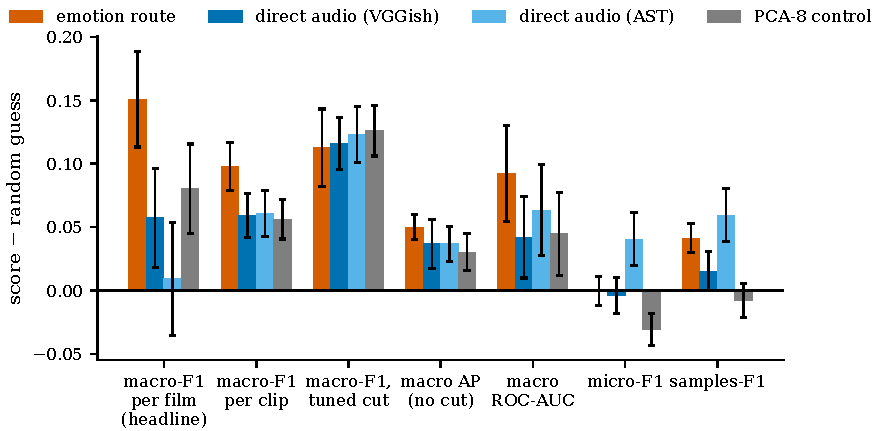
\includegraphics[width=\textwidth]{figures/metric_family.pdf}
  \caption{The four audio routes under seven metrics, as distance above the random guess (five genres, seed 42).}
  \label{fig:metric_family}
\end{figure}

In Figure~\ref{fig:metric_family}, each bar is a route's mean score over the ten repeats
minus the random guess of that metric; the whiskers are the standard deviation over the
repeats.

The metrics in the last block reward predicting the frequent genres and hardly care about
the rare ones. Under every one of them the most-frequent baseline, which predicts Drama
for every clip, beats every model: 0.571 micro-$F_1$ against at most 0.517, an
exact-match rate of 0.283 against at most 0.168, and a Hamming loss of
0.218 against at least 0.311. A metric under which a model that has learned
nothing ranks first is not a suitable headline for a question about genres such as Horror
and Comedy, which is why macro-$F_1$ is used. Among the metrics that weight genres equally,
the emotion route ranks first under both macro-$F_1$ scores and both threshold-free metrics.

The decision threshold matters more. When each genre's threshold is chosen to maximise
$F_1$ on the training fold, every route improves and, over clips, the four routes converge
to between 0.420 and 0.433, with the emotion route lowest. It is then no longer
ahead of VGGish ($-0.004$, $p=0.813$) or of the PCA-8 control ($-0.013$,
$p=0.422$). The two threshold-free metrics put it first, but not significantly (macro
average precision $+0.014$, $p=0.352$; macro ROC-AUC $+0.049$, $p=0.063$). Part of the
in-domain advantage at the default threshold is therefore an operating-point effect: the
emotion route places more clips of the rare genres above one half (macro recall 0.566
against 0.423 for VGGish, at precision 0.363 against 0.341). The fixed
threshold is not unfair, since the same rule is applied to every route, but per-genre
tuning \citep{lipton2014optimal} would narrow the gap. Film-level scoring uses the same cut
on averaged probabilities and inherits this caveat; thresholds were not tuned per film.
All transfer experiments use the default threshold as well.

\subsection{Stability and Reproducibility}

Figure~\ref{fig:stability_repeats} shows how the film-level scores vary over the ten
repeats and over five master seeds.

\begin{figure}[t]
  \centering
  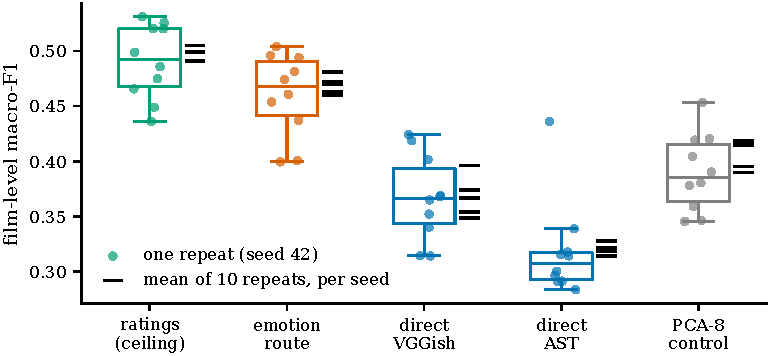
\includegraphics[width=\textwidth]{figures/stability_repeats.pdf}
  \caption{Stability of film-level macro-$F_1$ on the five-genre subset over repeats and master seeds.}
  \label{fig:stability_repeats}
\end{figure}

In Figure~\ref{fig:stability_repeats}, the coloured dots are the ten repeats under seed 42,
summarised by a box plot, and the black dashes are the ten-repeat means under each of the
five master seeds (42, 1, 2, 3, 4).

Three sources of variation were separated. Over the ten repeats, each of which assigns the
films to folds differently, the standard deviation of film-level macro-$F_1$ is between
0.034 and 0.045 (2.0 to 2.5 times the clip-level values of 0.016 to
0.019), because each genre's $F_1$ rests on a few films; the routes vary about equally
(the emotion route 0.038, VGGish 0.039, AST 0.045). Over the sample
of films, the bootstrap standard error is between 0.027 and 0.038. Over master seeds,
which change both the folds and the random forest of Stage~1, the ten-repeat mean moves by
0.005 to 0.019; the emotion route stays between 0.460 and 0.481, and its
lead is positive under every seed against VGGish ($+0.076$ to $+0.132$), AST
($+0.142$ to $+0.155$) and the PCA-8 control ($+0.051$ to $+0.071$). The PCA-8
control is itself ahead of VGGish under every seed ($+0.019$ to $+0.068$). Under seed
42 the re-run reproduces the per-repeat scores of the main analysis exactly. The numbers
are therefore stable against everything the code controls, and the remaining uncertainty
comes from the small number of films.

% =============================================================================
\section{Which Emotions Are Needed?}
\label{sec:app_ablation}

The ablation trains the genre classifier on the eight ground-truth ratings without the
derived features (all eight: 0.493 at film level), leaves each emotion out in turn, and
tests several theory-motivated subsets (Figure~\ref{fig:ablation}).

\begin{figure}[t]
  \centering
  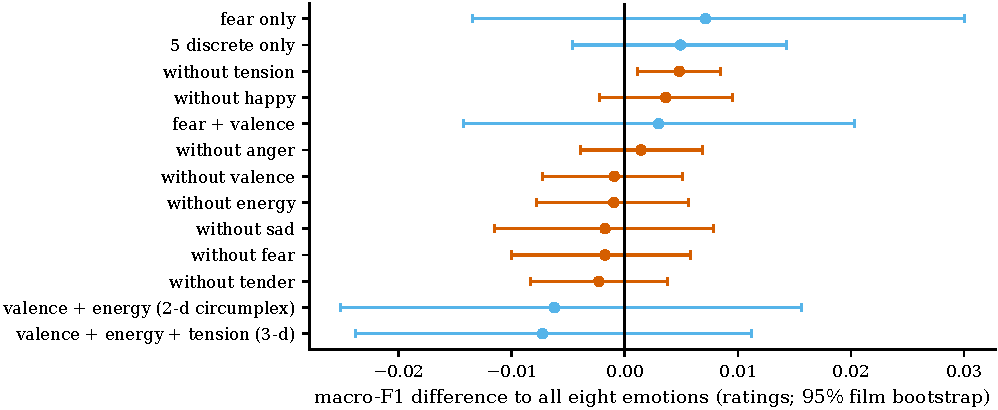
\includegraphics[width=\textwidth]{figures/ablation.pdf}
  \caption{Emotion ablation on the five-genre subset: change in film-level macro-$F_1$ relative to all eight emotions.}
  \label{fig:ablation}
\end{figure}

Each point in Figure~\ref{fig:ablation} is the difference to all eight emotions with a 95\,\%
bootstrap interval; orange points leave out one emotion, light blue points are subsets.

No single emotion is necessary: removing any one changes the score by at most
0.012. One of the eight changes reaches $p<0.05$: removing tension raises the score by 0.012 ($p=0.041$). With eight tests at the 5\,\% level one such result is roughly what chance produces, the Nadeau--Bengio test on the clip-level scores does not support it ($p=0.516$), and its direction is the opposite of what a necessary emotion would show. Smaller subsets lose a little, but not significantly: fear
alone reaches 0.475 ($p=0.345$), valence with energy 0.487 and the three dimensional
scales 0.479, so one to three emotions keep 96 to 99\,\% of the score of all
eight. The eight
ratings are strongly intercorrelated (fear rises with tension and falls with valence), and
the genre signal lies along essentially one threat-versus-warmth axis. Fear is the most
diagnostic emotion, but no emotion is necessary, and all eight are retained for
interpretability.

% =============================================================================
\section{The Waveform Representation}
\label{sec:app_waveform}

Used directly, wav2vec~2.0 is the weakest representation for genre (0.261 at film level),
behind each of the other five by 0.057 to 0.131. Routed through predicted
emotions, the same representation reaches 0.472, level with the VGGish pipeline and not
significantly below the ground-truth ceiling ($-0.018$, $p=0.546$). The gain over its direct
use, $+0.209$ [$+0.137$, $+0.277$], holds in all ten repeats ($p<0.001$; over clips $+0.086$,
Nadeau--Bengio $p=0.014$). The benefit of the emotion intermediate is therefore not tied
to one embedding, and it is largest where the underlying representation is weakest.

% =============================================================================
\section{All Eight Genres}
\label{sec:app_eight}

On the full eight-genre task (42 films), the pipeline reaches 0.349 [0.295,
0.389] at film level and the ratings 0.381, against a most-frequent baseline of
0.102 and a random guess of 0.226 (over clips: 0.317 and 0.328). The pipeline is
ahead of AST (0.242) by $+0.107$ ($p=<0.001$) and of the VGGish embedding it starts from
(0.257) by $+0.093$ ($p=0.001$), in all ten repeats. Over clips the Nadeau--Bengio test
gives $p=0.022$ against VGGish and $p=0.136$ against AST. The rarest
genres are almost never caught: Documentary, with two films, is never predicted correctly by
any route, and Biography (three films) reaches an $F_1$ of 0.11 in the emotion
route. Adventure, with ten films, is predicted poorly for its frequency (0.38
against 0.39 for Comedy with four films), in line with its missing emotional
signature (Section~\ref{sec:eval_signatures}).

% =============================================================================
\section{Blockbuster: Reproduction and Cue-Level Prediction}
\label{sec:app_blockbuster}

Table~\ref{tab:blockbuster_reference} compares the pipeline of this thesis with the
published results of \citet{ma2021computational} under their own protocol
(leave-one-film-out over the 110 films, macro-averaged precision, recall and $F_1$).

\begin{table}[tbp]
  \centering
  \caption{In-domain reference performance on the Blockbuster dataset (110 films, six genres).}
  \label{tab:blockbuster_reference}
  \small
  \setlength{\tabcolsep}{4pt}
  \begin{tabular}{lrrr}
    \toprule
    Model & Prec. & Rec. & $F_1$ \\
    \midrule
    \citeauthor{ma2021computational}: VGGish, single attention (their best) & 0.60 & 0.73 & 0.65 \\
    \citeauthor{ma2021computational}: VGGish, average pooling               & 0.55 & 0.78 & 0.62 \\
    \citeauthor{ma2021computational}: VGGish, $k$NN Simple-MI               & 0.64 & 0.59 & 0.61 \\
    \citeauthor{ma2021computational}: MIR, SVM Simple-MI                    & 0.60 & 0.52 & 0.56 \\
    \citeauthor{ma2021computational}: MIR, average pooling                  & 0.55 & 0.78 & 0.61 \\
    This thesis: VGGish + logistic regression                               & 0.569 & 0.705 & \textbf{0.620} \\
    \midrule
    Random guess (published / reproduced)     & 0.32 / 0.294 & 0.32 / 0.293 & 0.32 / 0.292 \\
    Plurality label set (published / reproduced) & 0.14 / 0.138 & 0.34 / 0.333 & 0.19 / 0.193 \\
    \bottomrule
  \end{tabular}
\end{table}

In Table~\ref{tab:blockbuster_reference}, the published values are quoted from
\citet{ma2021computational}, Table~4. The simple pipeline is within the range of their
VGGish models, and both of their baselines reproduce to within 0.03, so the classifier is
validated against an external result before it is used for transfer. Under the repeated
protocol of Figure~\ref{fig:blockbuster_cv}, the learned embedding does not beat the full
set of 140 hand-crafted MIR features ($+0.009$, $p=0.787$); an earlier, larger gap came
from comparing it with the 78 MFCC-family features only ($+0.077$, $p=0.062$).

A Blockbuster film consists of individually scored cues (4664 in total, a median of 39 per
film, with a median length of 19\,s), and a cue is the same kind of object as an Eerola
clip. Predicting the emotions of each cue and averaging them afterwards outperforms
predicting them once from the film-average embedding: 0.616 against 0.557
in-domain ($+0.059$, Nadeau--Bengio $p=0.020$, in 92\,\% of the folds), and
only slightly in the zero-shot setting (0.508 against 0.502). Applying the emotion
model at the granularity it was trained on is thus part of the method. The multi-instance structure
itself adds little, since a majority vote over cues is not significantly better than
averaging the cues ($+0.028$, $p=0.388$).

% =============================================================================
\section{Error Analysis}
\label{sec:app_errors}

The genre classifier uses class-balanced weights so that rare genres are not ignored, and
this leads to over-prediction: on the eight-genre task, under the earlier single-run
protocol, it assigned 3.55 genres per clip on average against 1.87 true ones. Raising a
single decision threshold above 0.5 makes macro-$F_1$ worse rather than better, because it
removes the positive predictions of the rare, distinctive genres first; a threshold tuned
per genre is a different matter (Section~\ref{sec:eval_robustness}). A learning curve, in
which the models were trained on growing fractions of the films, was still rising at the
full dataset size for both the emotion features and the AST embedding, so performance is
limited by the amount of data as well as by the signal. Finally, grouping by film matters:
under an ungrouped split the AST baseline reaches 0.44 instead of 0.23
(clip-level macro-$F_1$, eight genres, single untuned five-fold run), because it can
recognise the film rather than the genre, while the emotion features gain much less from
the same leakage.
